\chapter{Methodology}
\label{ch3}
Despite of its provable strength, \gls{bananas} assumes a Gaussian distribution for measuring uncertainty. However, this assumption does not necessarily hold in real world. To mitigate the potential limitations caused by inaccurate uncertainty estimates, this work proposes a new framework that integrates a conformal prediction-based uncertainty calibration process into \gls{bananas} in an online setting. 

An algorithm outlining the overall procedure of \gls{bananascp} is presented in Section \ref{sec:overview}, followed by detailed descriptions of each methodological step. Section \ref{sec:cp} presents different conformal predictions algorithms to be explored. Next in Section \ref{sec:distest}, methods for the estimation and evaluation of the conditional distribution of each candidate architecture are discussed. Finally, in Section \ref{sec:acq} we introduce how the calibrated distribution can be combined with different acquisition functions and acquisition search strategies in the Bayesian optimization process.


\section{The BANANAS--CP Framework}
\label{sec:overview}

Refer to Section {\ref{sec:bananas} for a detailed introduction of the original \gls{bananas} algorithm. In this section, we emphasis the key ideas of the uncertainty calibration mechanism, which corresponds to Step 1 to 6 of the inner iteration in Algorithm {\ref{alg:OCP}.

\begin{algorithm}[htbp]
  \caption{The BANANAS--CP Framework}
  \label{alg:OCP}
  \begin{algorithmic}[1]
    \textbf{Input - NAS parameters:}
    search space $\mathcal{A}$, evaluation dataset $\mathcal{D}$, exploration budget $T$, 
    the number of initially sampled architectures $t_{0}$, acquisition function $\phi$, surrogate model $\mathcal{M}$ that approximates the true objective function, function $\myfunc{f(\cdot)}$ returning validation error of an architecture after training. \newline
    \textbf{Input - Calibration parameters:} a function $\myfunc{C(\cdot)$ to create calibration set, a non-conformity score function $\myfunc{s(\cdot)}$, and an array of desired quantile levels $q$. \vskip
    \vspace{0.7em}
    \STATE Draw $t_{0}$ architectures {$\{a_{1}, a_{2},..., a_{t_{0}}\}$} uniformly at random from $\mathcal{A}$ and train each individual architecture on $\mathcal{D}$.
    \vspace{0.3em}
   	\STATE $\mathcal{A}_{t_{0}} \leftarrow{\{a_{1}, a_{2},..., a_{t_{0}}\}$},
   	\vspace{0.3em}	
    \FOR {$t$ in $t_{0}+1,...,T$}
    	\begin{enumerate}
    	    \itemsep0em 
			\item Apply $\myfunc{C(\cdot)$ and split all evaluated architectures into two disjoint datasets; use them as a training set $\mathcal{A}_{t, train}$, and a calibration set $\mathcal{A}_{t, cal}$.
			\item Train the surrogate model $\mathcal{M}_{t}$ on $\{a, \myfunc{f(a)}\}, a \in \mathcal{A}_{t, train}$ using the path encoding to represent each architecture. 
			\item Compute the conformity scores $\myfunc{s}$ on $\mathcal{A}_{t, cal}$.
			\item Generate a set of candidate architectures from $\mathcal{A}$. 
			\FOR {each $a_{i}$ in candidates}
				\begin{enumerate}
				\itemsep0em 
				\item Estimate the value for each quantile level $q_i$ in $q$ and calibrate using conformity scores computed in the previous step, with $q_i$ implying a mis-coverage rate $2q_i$ or $2(1-q_i)$ for conformal prediction.
				\item Fit a distribution $F_{i}$ based on the estimated quantile values.
				\item Compute the acquisition score $\myfunc{\phi(a_{i})}$.
				\end{enumerate}
			\ENDFOR
			
			\item Denote $a_{t}$ as the candidate architecture with maximum $\myfunc{\phi(a)}$; evaluate $\myfunc{f(a_{t})}$.
			\item $\mathcal{A}_{t} \leftarrow{\mathcal{A}_{t-1} \cup \{{a_{t}\}}$
		\end{enumerate}
    \ENDFOR 
    \STATE \textbf{Output:} $a^{*}=\operatorname*{argmax}_{t=1,...,T} f(a_{t})$    
  \end{algorithmic}
  \end{algorithm}

Bayesian optimization is a form of sequential decision-making task. In the applications of neural architecture search, the typical goal is to find the architecture that has the best evaluation performance on a fixed dataset under a given search budget. At each ietration $t$, a surrogate model is trained on all architectures evaluated at step $\{0, 1, 2..., t-1\}$ and their associated validation accuracies, to predict the scores of unseen architectures for the next search.

In the standard \gls{bananas} setting, the surrogate model is an ensemble of $m$ feedforward neural networks, typically $m=5$. At iteration $t$, a set of candidate architectures is sampled, and a conditional Gaussian distribution is estimated for each candidate based on the ensemble predictions, as expressed below:
\vspace{1em}
\begin{equation}
\hat{f}(a) \sim \mathcal{N} \left( 
\frac{1}{m} \sum_{i=1}^{m} f_i(a),\ 
\sqrt{\frac{1}{m} \sum_{i=1}^{m} \left(f_i(a) - \frac{1}{m} \sum_{j=1}^{m} f_j(a) \right)^2}
\right)
\label{eq:ensemble_gaussian}
\vspace{0.7em}
\end{equation}
\noindent
where $a$ denotes an architecture sampled from the search space, and $f_i(a)$ is the predicted accuracy from the $i$-th base learner of the ensemble for architecture $a$.

In the \gls{bananascp} framework, a key distinction is that all architectures evaluated at step $\{0, 1, 2..., t-1\}$ are divided disjointly into a training set and a calibration set. Then, the surrogate model is trained exclusively using samples in the training set, while the calibration set is used to compute conformity scores for quantile calibration. In practice, at each iteration $t$, the surrogate model estimates a conditional distribution $\hat{F}$ for an unseen architecture over its validation accuracy on the target dataset, either based on a specific distribution assumption or a probabilistically-interpretable modeling approach, e.g. quantile regression. Following the definition in \cite{deshpande2024online, pmlr-v80-kuleshov18a}, calibration means that for any quantile level $p\in [0, 1]$, the empirical fraction of data-points below the $p$-th percentile of the predicted distribution $\hat{F}$ should converge to $p$ as the sample size goes to infinity. For example, if p = 80\%, then the 80th percentile of $\hat{F}$ is set to the threshold value such that 80\% of previously evaluated architectures fall below, thereby aligning with the empirical coverage. In an online setting, the objective of the calibration process can be defined as:

\begin{equation}
\frac{1}{T} \sum_{t=1}^{T} \mathbb{I} \left\{ y_t \leq Q_t(p) \right\} \rightarrow p \quad \text{for all } p \in [0,1]
\vspace{1em}
\end{equation}
as $t \rightarrow \infty$, where $\mathbb{I}$ is the indicator function and $Q_t(p)$ represents the distribution $\hat{F}$ in the format of quantile function \cite{deshpande2024online, pmlr-v80-kuleshov18a}. 

Next, as in the standard  Bayesian optimization process, the acquisition function picks the architecture for the next evaluation based on the conditional distribution of all sampled candidates.

\section{Uncertainty Calibration Algorithms}
\label{sec:cp}
As reviewed in Section \ref{sec: reviewCP}, numerous conformal prediction algorithms have been proposed in recent research. This work identifies several approaches applicable in \gls{nas} for building a calibration set and computing conformity scores. This section provides an overview of these splitting strategies, as well as the conformity scoring functions that are commonly used for regression problems.
\subsection{Split Conformal Prediction}
\label{sec:scp}
To begin, a natural choice for a baseline calibration strategy is the \gls{scp}. In this section, we start by introducing the standard \gls{scp} procedure, then proceed with the adaptions required to incorporate it into the \gls{bananascp} framework. 

Implementation steps of \gls{scp} are summarized in Algorithm \ref{alg:SCP}. Imagine a regression task where the non-conformity level is measured by the absolute residual, i.e. $|y_i - \hat{y}(x_i)|$. In this case, the algorithm produces a prediction interval for the test point with a width of $\left[\hat{y}_{test} - \hat{q}\;,\; \hat{y}_{test} + \hat{q}\right]$, where $\hat{q}$ is the conformity threshold as defined in line 6 in.

\begin{algorithm}[htbp]
  \caption{Split Conformal Prediction}
  \label{alg:SCP}
  \begin{algorithmic}[1]
    \textbf{Input:} 
    A set of observations $\{(x_{i}, y_{i})\}_{i=1}^n$, a prediction algorithm $h(\cdot)$, a non-conformity measure $\myfunc{s(\cdot)}$, nominal mis-coverage rate $\tau$, fraction of data assigned to the training set $p_{train}$, test data $x_{n+1}$. \vskip
    \textbf{Output:} a prediction set $\mathcal{C}_{\tau}(x_{n+1})}$ that covers $y_{n+1}$ with probability $1-\tau$. \vskip
    \vspace{0.3em}
    \STATE Allocate at random a proportion of $p_{train}$ of the observations to the training set $\mathcal{D}_{train}$ and use the rest for calibration $\mathcal{D}_{cal}$.
    \STATE Train the point predictor $h(\cdot)$ on $\mathcal{D}_{train}$.
    \STATE Initialise a scoring set $S=\emptyset$
    \FOR {$(x_i, y_i)$ in $\mathcal{D}_{cal}$}
		$S \gets S \cup \{s(h(x_i), y_i)\}$
	\ENDFOR
	\STATE Return $\mathcal{C}_{\tau}(x_{n+1}) \leftarrow \{y \,|\, s((h(x_{n+1}), y) \leq q\}$, where $q$ is the $\lceil(1-\tau)(n_s+1)\rceil$-th smallest value of $S$, with $n_s = |S|$.
    \end{algorithmic}
\end{algorithm}

In this work, we explore \gls{scp} in combination with different prediction algorithms. First, we follow the settings in \gls{bananas} and use an ensemble of five \gls{fnns} as the underlying surrogate model. In this case, note that the bounds of the prediction set as identified in Algorithm \ref{alg:SCP} should not be simply interpreted as the quantile values of a distribution, since the prediction algorithm does not directly model the $\tau$-quantile of the variable Y, i.e., ${Q_Y(\tau)= F_{Y}^{-1}(\tau) = \inf \left\{y\colon F_{Y}(y)\geq \tau\}$, with $\tau \in [0, 1]}$ denoting a quantile level and $F_Y$ its cumulative distribution function. Thus, the ensemble predictor must be used in conjunction with a valid distribution assumption to obtain valid quantile values. Motivated by the goal of achieving a completely distribution-agnostic solution, we next replace the ensemble model with a quantile regressor that directly models the quantiles of a distribution. In the remainder of this section, we discuss the configurations designated for each prediction algorithm. 
\vspace{0.7em}
\begin{description}[leftmargin=0cm, listparindent=\parindent]
	\item [Ensemble Predictor] Following the settings in the original \gls{bananas}, an ensemble by default consists of five neural networks, where each neural network is a fully-connected multi-layer perceptron with 20 layers of width 20. The neural networks are trained by minimizing the mean absolute error (MAE), using the Adam optimizer with a learning rate of 0.01. In parallel to \gls{bananas}, we assume that the validation accuracy of each unseen candidate architecture $a$ follows a Gaussian distribution, which is parameterized by the predictive mean ($\hat{\mu}$) and standard deviation ($\hat{\sigma}$) provided by the ensemble model, as demonstrated in equation \ref{eq:ensemble_gaussian}. For a specific significance level $\alpha$ (suppose $\alpha<0.5$), the central quantile interval can be written as:
		\vspace{0.7em}
		\begin{equation}	
		\left[	
		\hat{\mu} - \Phi^{-1}_{1 - \alpha/2} \cdot \hat{\sigma}	\; ,\; 
		\hat{\mu} + \Phi^{-1}_{1 - \alpha/2} \cdot \hat{\sigma}
			\right]
		\label{math:gaussianinterval}
		\vspace{0.5em}
		\end{equation}
		
	\noindent	
	where $\Phi^{-1}_{1 - \alpha/2}$ denotes the $(1-\frac{\alpha}{2})$-th quantile of the standard normal distribution. \\
	
	Now, take a closer look at the formula \ref{math:gaussianinterval} and recall the example based on the absolute residuals, which is presented earlier in this section. We observe that the confidence interval under the Gaussian assumption takes a close form to the prediction interval produced by \gls{cp} when the conformity scoring function is exactly chosen as:
		\vspace{0.7em}
		\begin{equation}
			s(\cdot) = \frac{|y_i - \hat{y}(x_i)|}{\hat\sigma(x_i)}
		\label{cpscore}
		\vspace{0.7em}
		\end{equation}
	
	Hence, the bounds of the \gls{cp}-derived prediction interval can be \textit{approximately} interpreted as empirically calibrated quantile estimates under the Gaussian assumption, provided that the conformity scoring function is chosen appropriately. Note that the absolute residual can be seen as a special case of equation \ref{cpscore} as well, where the empirical standard deviation estimate is disregarded and fixed at one. In fact, this scaled absolute residual (equation \ref{cpscore}) is a popular choice for measuring conformity in practice. Ideally, we would like the \gls{cp}-derived prediction interval also demonstrates local adaptivity, i.e., the prediction interval should have a larger width if the prediction task is difficult and smaller otherwise. The scaled absolute residual accounts for heteroskedasticity and is able to adjust the width of the prediction band by multiplying the standard deviation estimate. In contrast, the band produced with a pure residual score has constant-width everywhere regardless of the input, which limits its effectiveness in application. Therefore, in this work, we use the scaled absolute residual as the conformity scoring function for ensemble predictors, unless otherwise specified.
	\vspace{0.7em}
	\item [Quantile Regressor] We now explain how a quantile regressor can be leveraged to build a probabilistic surrogate for Bayesian optimization. We follow the methods established previously in \cite{romano2019conformalized, salinas2023optimizing}.
	
	
	We start with a brief introduction into the quantile regression \cite{koenker1978regression}. Suppose $(x, y) \sim F$ denote data drawn from a joint distribution that is characterized by its cumulative distribution function $F$, the aim of the conditional quantile regression is to estimate a given quantile of the conditional distribution of $Y$ given $X=x$. The conditional quantile function for $\tau$-quantile is:
		\begin{equation}
			Q(\tau) = \inf \left\{ y \in \mathbb{R} : \mathbb{P}(Y \leq y \mid X) \geq \tau \right\}
		\label{quantilefunc}
		\end{equation}
		
	\noindent and can be estimated by minimizing the Pinball loss on the training data \cite{koenker1978regression}:
		\begin{equation}
			\ell_\tau(y, \hat{y}) = 
			\begin{cases}
			\tau (y - \hat{y}), & \text{if } y \geq \hat{y} \\
			(1 - \tau)(\hat{y} - y), & \text{otherwise}
			\end{cases}
		\label{pinballloss}
		\end{equation}
		
	\noindent where $\hat{y}$ is the predicted quantile value.	 As illustrated in Figure \ref{fig:CQR}, the Pinball loss is asymmetric and the intuition behind is that under-estimate and over-estimate receive different penalties across quantiles. 	For instance, if $\tau=0.9$, then we would expect that empirically 90\% of observations should fall below the prediction. In this case, the loss function places a higher penalty for underestimate.	
	
	Quantile regression in the \gls{bananascp} framework is implemented by training a dedicated neural network for each quantile level $\tau_j$ in the quantile array as defined in Algorithm \ref{alg:OCP} using the corresponding Pinball loss $\ell_{\tau_j}(y, \hat{y})$. 
	
	 While quantile regression can model the shape of any continuous distribution given enough data, the predictions are not guaranteed to be well calibrated in practice. In fact, it is not uncommon that quantile regression generates non-monotonic predictions, a phenomenon referred as quantile crossing. To address this issue, we apply a post-hoc calibration upon the predicted quantiles using the \gls{cqr} from \cite{romano2019conformalized}. This method consists of a novel conformity score tailored for quantile estimation and the key idea of calibration is to apply quantile-aware offsets, which are computed on the calibration set, on the original predicted quantiles. 
		 
	 \begin{figure}[t]	
		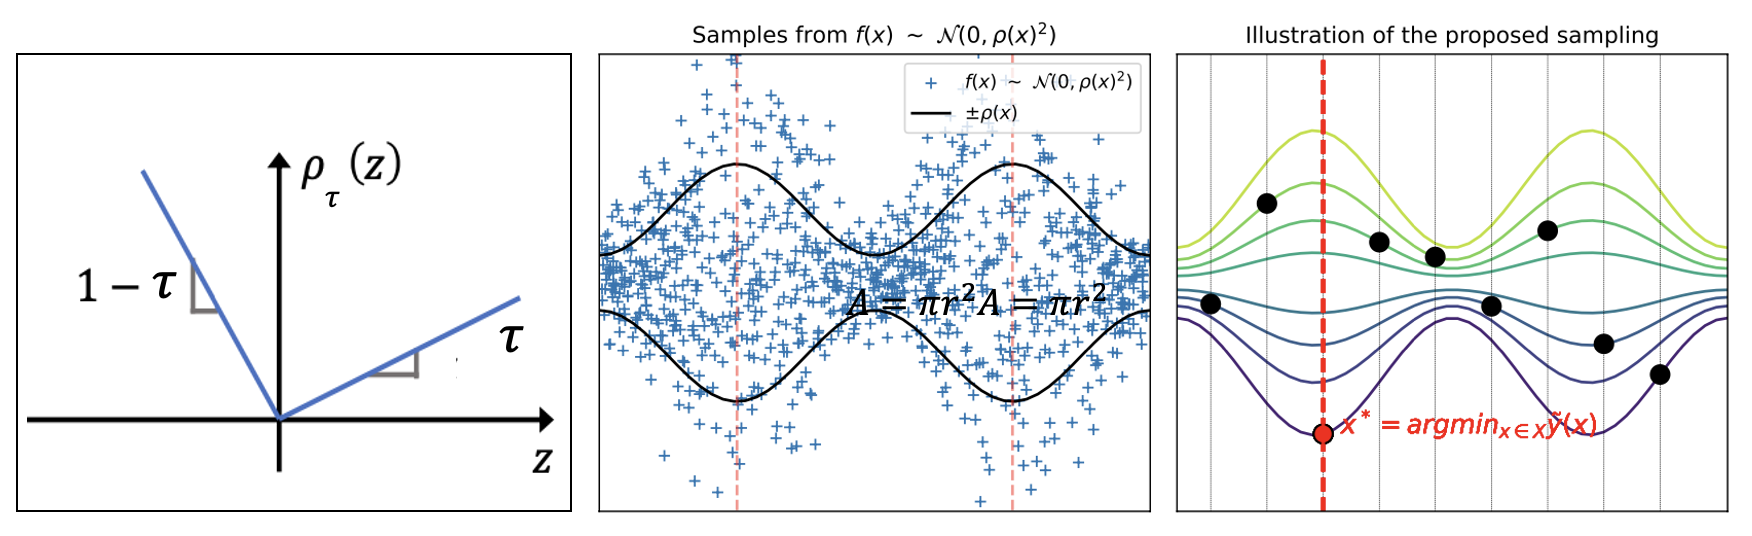
\includegraphics[scale=0.56]{figs/pinball_loss_and_CQR.png}
		\refstepcounter{figure}
   		\addcontentsline{lof}{figure}{Figure~\thefigure: Pinball loss and CQR within Bayesian optimization}
		\label{fig:CQR}
		{\small \textit{Figure \ref{fig:CQR}:} Visualization of the Pinball loss function, where $z=y - \hat{y}$ \cite{romano2019conformalized} (left); Samples from a synthetic heteroskedastic function (middle) and  the sampling procedure based on $|q| = 8$ predicted quantiles \cite{salinas2023optimizing} (right).
		}
	\end{figure}
	 
	 A close work is \cite{salinas2023optimizing} that employs \gls{cqr} to obtain quantiles with robust coverage during hyperparameter tuning via Bayesian optimization. Specifically, the calibrated quantiles are used to select the candidate for the next search, where a set of candidates is first sampled uniformly at random, and then for each of those candidates a random quantile is simply picked and is treated as the acquisition score (Figure \ref{fig:CQR}). We follow their notation and interpretation in defining the conformity score for a quantile surrogate:  
	 
	 \begin{equation}
		E_i = \max \big\{\hat{q}_{\tau_j}(x_i) - y_i, \; y_i - \hat{q}_{1-\tau_j}(x_i) \big\}
	 \vspace{0.7em}
	 \label{scoreCQR}
	 \end{equation}
	 
	 \noindent where $\hat{q}_{\tau}(x_i)$ denotes the predicted $\tau$-quantile at $x_i$. Note that the sign of the score is positive when the target $y_i$ is outside of the interval and negative when the target falls inside the predicted interval. This allows the conformity score to account for both overcoverage and undercoverage cases. In addition, the score amplitude always measures the distance to the closer quantile between $\hat{q}_{\tau_j}(x_i)$ and $\hat{q}_{1-\tau_j}(x_i)$ \cite{romano2019conformalized, salinas2023optimizing}.	 

\end{description}


\subsection{Conformal Prediction with Cross-validation}}
Solving a NAS problem is usually computationally expensive, as each neural architecture evaluation incurs the cost of fully training and validating the underlying model on the target dataset. Motivated by the fact that \gls{nas} based on Bayesian optimization is typically allocated with a budget of 100 to 200 epochs, an additional heuristic for constructing the calibration set via cross-validation (hereafter: \gls{cvcp}) is employed to avoid reducing the sample size for obtaining a holdout set as performed in \gls{scp}.

The \gls{cvcp} method is a natural extension of \gls{scp} and is first formally presented in  \cite{vovk2015cross}. At each step, the evaluated architectures are devided at random into $K$ folds. A dedicated surrogate model is trained on $K-1$ folds, while the remaining one is used as the calibration set to calculate the conformity scores. This process is repeated for $K$ times over each individual fold. Finally, conformity scores from all calibration folds are combined to form the overall calibration set, on which the quantile is computed to determine the calibration offset. For an unseen data point, the prediction is obtained by aggregating the predictions of the $K$ trained models, e.g., by taking the average of the model outputs.  Algorithm \ref{alg:CVCP} summarizes this procedure. 

\vspace{1em}
\begin{algorithm}[t]
  \caption{Conformal Prediction with Cross-validation}
  \label{alg:CVCP}
  \begin{algorithmic}[1]
    \textbf{Input:} 
    A set of observations $\{(x_{i}, y_{i})\}_{i=1}^n$, number of folds $K$, a prediction algorithm $h(\cdot)$, a non-conformity measure $\myfunc{s(\cdot)}$, nominal mis-coverage rate $\tau$, test data $x_{n+1}$. \vskip
    \textbf{Output:} a prediction set $\mathcal{C}_{\tau}(x_{n+1})}$ that covers $y_{n+1}$ with probability $1-\tau$. \vskip
    \vspace{0.5em}
    \STATE Initialise a conformity scoring set $S=\emptyset$
    \STATE Split the observations $\{(x_{i}, y_{i})\}_{i=1}^n$ into $K$ folds at random. $I_k$ denotes the index set containing indices of samples in the $k$-th fold.
    \FOR {$k$ in 1, 2, ..., K}
		\begin{enumerate}
    		\item Train $\hat{h}_{-k}(\cdot)$ on $\{(x_{i}, y_{i}) \mid i \notin I_k\}$
    		\item Compute conformity score on the $k$-th fold $S_k=\{s((\hat{h}_{-k}(x_{i}), y_i) \mid i \in I_k\}$
    		\item $S \leftarrow{S \cup S_k}$
    	\end{enumerate}
   	\ENDFOR
	\STATE Predict $x_{n+1}$: $h(x_{n+1}) \leftarrow aggregate(\{\hat{h}_{-1}(x_{n+1}), ..., \hat{h}_{-K}(x_{n+1})\})$ 
	\STATE Return $\mathcal{C}_{\tau}(x_{n+1}) \leftarrow \{y \,|\, s((h(x_{n+1}), y) \leq q\}$, where $q$ is the $\lceil(1-\tau)(n_s+1)\rceil$-th smallest value of $S$, with $n_s = |S|$.
    \end{algorithmic}
\end{algorithm}

Note that the only distinction between \gls{scp} and \gls{cvcp} is how the calibration set is constructed. Since it does not place any additional restriction on the choices of the underlying surrogate, \gls{cvcp} can be applied in conjunction with either ensemble predictor or quantile regressor in the same way as \gls{scp}. See Section \ref{sec:scp} for detailed configurations.

\subsection{Conformal Prediction with Bootstrapping}
Inspired by the fact that \gls{bananas} is built on an ensemble surrogate, we further explore incorporating Jackknife+-after-boostrap \cite{kim2020predictive}, a wrapper for predictive inference designed specifically for use with ensemble learners, into the calibration step (hereafter: \gls{btcp}).

In contrast to fitting $m$ neural networks on the same training data with different random weights initializations, as applied in the \gls{bananas} framework, a different technique to build an ensemble model is via bootstrapping. Specifically, the ensemble method starts by creating multiple training datasets by resampling the available data points with replacement. In the next step, multiple models are trained on each of the bootstrapped subsets, and their predictions are aggregated to produce the single final prediction \cite{breiman96}. This technique offers more accurate and stable estimates than a single model and has shown superior performance in application.

\begin{algorithm}[t]
  \caption{Conformal Prediction with Bootstrapping}
  \label{alg:BtCP}
  \begin{algorithmic}[1]
    \textbf{Input:} 
    A set of observations $\{(x_{i}, y_{i})\}_{i=1}^n$, number of bootstraps $B$, a prediction algorithm $h(\cdot)$, a non-conformity measure $\myfunc{s(\cdot)}$, nominal mis-coverage rate $\tau$, test data $x_{n+1}$. \vskip
    \textbf{Output:} a prediction set $\mathcal{C}_{\tau}(x_{n+1})}$ that covers $y_{n+1}$ with probability $1-\tau$. \vskip
    \vspace{0.5em}
    \STATE Sample all available data with replacement and create $B$ subsets. $I_b$ denotes the indices of data points included in the $b$-th sample.
    \STATE Train $\hat{h}_{b}(\cdot)$ on $\{(x_{i}, y_{i}) \mid i \in I_b\}$ for $b$ in 1, 2, ..., B
    \STATE Initialise a conformity scoring set $S=\emptyset$
    \FOR {$i$ in 1, 2, ..., n}
    	\begin{enumerate}
    		\STATE Initialize an empty for leave-one-out estimates $LOO_i=\emptyset$
    		\STATE For {$b$ in 1, 2, ..., B},  if {$i$ \notin \; $I_b$}\;: $LOO_i \leftarrow{LOO_i \cup \hat{h}_b(x_i)}$ 
			\STATE S \gets S \cup s\big(aggregate(LOO_i),\; y_i\big)
		\end{enumerate}
    \ENDFOR
	\STATE Predict $x_{n+1}$: $h(x_{n+1}) \leftarrow aggregate(\{\hat{h}_{1}(x_{n+1}), ..., \hat{h}_{B}(x_{n+1})\})$ 
	\STATE Return $\mathcal{C}_{\tau}(x_{n+1}) \leftarrow \{y \,|\, s((h(x_{n+1}), y) \leq q\}$, where $q$ is the $\lceil(1-\tau)(n_s+1)\rceil$-th smallest value of $S$, with $n_s = |S|$.
    \end{algorithmic}
\end{algorithm}

Jackknife+ is a type of \gls{cp} algorithm that is closely related to the \gls{loo} method \cite{barber2020jackknife}. Given a set of observations $\{(x_{i}, y_{i})\}_{i=1}^n$, the idea is to fit an \gls{loo} estimator $\hat{h}_{-i}$ using all available data except for the $i$-th sample, and this process iterates over all individual samples. Then, the predictive interval around the $i$-th point is obtained by offsetting the prediction from $\hat{h}_{-i}(x_i)$ with the quantile of all \gls{loo} conformity scores.  Equivalently, Jackknife+ can be viewed as a special case of \gls{cvcp} when the number of folds is exactly set to $K=n$.

Jackknife+-after-boostrap \cite{kim2020predictive} integrates both approaches and provides a cost-efficient wrapper by leveraging only the available bootstrapped sets and their corresponding fitted models, thereby avoiding re-fitting ensembles on each individual bootstrapped sample. \cite{pmlr-v139-xu21h} extends this method to online setting and proves its efficiency for time-series data. In contrast to the \gls{cp} algorithms described in earlier sections, \gls{btcp} requires no data splitting because sampling with replacement automatically creates holdout sets. Training the bootstrap ensemble on random subsets from the full data also reduces the chance of overfitting.

Implementation of \gls{btcp} is shown in Algorithm \ref{alg:BtCP}. Noteably, if a particular  data point appears in all bootstrapped samples, it is then excluded from the computation of conformity scores since it has no associated \gls{loo} estimator. In \gls{btcp}, the absolute residual is mainly used for measuring conformity, due to potentially insufficient \gls{loo} outputs for standard deviation estimation, i.e., $LOO_i$ in Algorithm \ref{alg:BtCP} might have fewer than two points. Specifically, \gls{btcp} is only applied with the ensemble model. This concludes our experiment setups and the \gls{bananascp} framework is finally evaluated under five various predictor+CP configurations.


\section{Distribution Estimation}
\label{sec:distest}
As described in Section \ref{sec:bananas}, Bayesian optimization generally relies on a continuous posterior distribution at $X=x$ to obtain the acquisition score. Here, we denote by $F_t(x)$ the \gls{cdf} of the posterior distribution of the data point $x$ at step $t$. In the context of NAS, where the target variable is assumed to be continuous and real-valued, the distribution can be represented by the inverse of its \gls{cdf}, or quantile function without loss of generality, i.e. $Q_{t}(x) = F^{-1}_{t}(x)$. 

In the \gls{bananascp} framework, as outlined in Algorithm \ref{alg:OCP}, we are able to generate calibrated quantile estimates for a finite set of discrete quantile levels. Intuitively, assuming the quantiles estimates are accurate, increasing the granularity of quantile levels should lead to a more accurate approximation of the underlying continuous distribution. However, it is computationally prohibited to estimate an infinite number of quantiles in practice, especially with significantly limited training data. Therefore, we propose an approach for constructing a continuous distribution from discrete quantile estimates with mild assumption. Specifically, the distribution estimator is defined as:

\vspace{0.5em}
\begin{description}[leftmargin=0cm, listparindent=\parindent]
\item[Definition] Let $\{q_i\}_{i=1}^n$ be a quantile of percentile levels such that $0<q_1<q_2, ..., <q_n<1$, and $\{v_i\}_{i=1}^n$ are the corresponding quantiles, i.e., $F^{-1}(q_i)=v_i$, the empirical \gls{cdf} of the distributions $\hat{F}$ is constructed by applying linear interpolation between adjacent quantiles. Consequently, the \gls{pdf} of a specific interval $\left(v_a, v_b\right), a,b \in \{1,..., n\}$ and $a<b$ is:
\vspace{0.5em}
\[
PDF(x) = \frac{q_b - q_a}{v_b - v_a}, \quad & \text{if } x \in (v_a, v_b) \\
\]

\vspace{1em}
\item[Diagnosis Analysis] To assess the validity of this approach, we first perform a diagnosis analysis using synthetic datasets generated by a left-skewed Gaussian distribution, which we believe resembles the true underlying distribution of the validation performances of architectures in a search space. The experiments on the synthetic data are intended to reflect the comparisons in a real \gls{nas} application, therefore two kinds of distribution estimators are examined: a Gaussian estimator and a linear-interpolation based quantile estimator. The analysis is repeated with different parameterizations, e.g, the number of quantiles, or the size of the samples, etc.

Table \ref{table:distest} reports the performance of three distribution estimators on synthetic datasets with various sample sizes. In particular, the linear-interpolation based quantile estimator is evaluated under 10 and 20 quantile levels, and the quantile estimates for interpolation are obtained by taking the empirical quantiles of the sample data. The estimation performance is assessed using the mean, standard deviation and Kullback–Leibler (KL) divergence \cite{kullback1951information}. For each sample size, we run 50 trials and aggregate the metrics over the trials to reduce the effects of randomness. Results in Table \ref{table:distest} indicate that the linear-interpolation based quantile estimator offers a better approximation to an asymmetric distribution than a Normal distribution, and increasing the number of quantile levels leads to improved approximation performance, provided with sufficient data. However, a caveat is that quantile-based estimation tends to produce biased standard deviation estimates, which may lead to undesired effect.

Having considered the behaviors of the various acquisition functions employed in the real \gls{bananascp} application (see Section \ref{sec:acq}), we additionally present several visualizations based on a synthetic dataset with 150 samples (Figure \ref{fig:distest10}, Figure \ref{fig:distest20}) to confirm the shapes of the estimated distributions are not significantly deviated from that of the true underlying distribution, thereby assuring the effectiveness of the acquisition functions.

\vspace{1em}
\item[Evaluation Metrics] Within the \gls{bananascp} framework, the calibration quality at a specific epoch is measured by the \gls{rmsce} \cite{pmlr-v80-kuleshov18a}. Suppose $\hat{F}^{-1}_t$ is the \gls{cdf} of the distribution estimated at the  $t$-th step and $y_t$ is the true value revealed after the estimation, consider a sequence of $\{(\hat{F}^{-1}_t, y_t)\}_{t=1}^T$ that represents a neural architecture search process after $T$ epochs, the calibration error at the $T$-th epoch is defined as:
	\vspace{0.5em}
	\begin{equation}
	\text{RMSCE} \left( \hat{F}^{-1}_1, y_1, \dots, \hat{F}^{-1}_T, y_T \right) = \sum_{j=1}^m w_j \left( p_j - \hat{p}_j \right)^2
	\label{rmsce}
	\end{equation}

	\[
	\text{with} \quad
	\hat{p}_j = \frac{\left| \left\{ y_t \;\middle|\; \hat{F}^{-1}_t(y_t) \le p_j,\; t = 1, 2, \dots, T \right\} \right|}{T}
	\]

\noindent where $m$ represents the number of discrete quantile levels and the scalars $w_j$ are  quantile weights. For simplicity, we adopt  $w_j=1, \forall j \in[0,1]$ in this work. Alternatively, calibration errors of the quantiles can be weighted by the number of observations falling into the corresponding intervals. Note that calibration errors calculated with different numbers of quantiles are not directly comparable. In general, increasing the number of quantiles tends to lead to larger calibration errors.	
\end{description}


\begin{table}[htbp]
\centering
\refstepcounter{table}
\addcontentsline{lot}{table}{Table~\thetable: Statistical Comparison of Distribution Estimators}

\parbox{\linewidth}{
  {\small \textit{Table \ref{table:distest}}: Statistical metrics of distributions estimated by three methods on synthetic datasets with sample size ranging from 50 to 500. For each method and sample size, the mean, standard deviation, and KL divergence are reported to assess the estimation performance.}  
}

\label{table:distest}
\vspace{2em}
\begin{tabular}{llc>{\centering\arraybackslash}p{2.5cm}c}
\toprule
\textbf{Sample Size} & \textbf{Estimator} & \textbf{Mean} & \textbf{Standard Deviation} & \textbf{KL Divergence} \\
\midrule
\multirow{50}  & Gaussian            & -0.7985 & 0.6005 & 0.5727 \\
               & Quantile ($|q|=10$) & -0.7481 & 0.5503 & 0.1646 \\
               & Quantile ($|q|=20$) & -0.7440 & 0.5536 & 0.2928 \\
\midrule
\multirow{100} & Gaussian            & -0.7989 & 0.6145 & 0.6181 \\
               & Quantile ($|q|=10$) & -0.7744 & 0.5941 & 0.0953 \\
               & Quantile ($|q|=20$) & -0.7654 & 0.5798 & 0.1297 \\       
\midrule
\multirow{150} & Gaussian            & -0.7986 & 0.6100 & 0.5977 \\
               & Quantile ($|q|=10$) & -0.7860 & 0.6133 & 0.0811 \\
               & Quantile ($|q|=20$) & -0.7791 & 0.5950 & 0.0948 \\
\midrule    
\multirow{200} & Gaussian            & -0.7969 & 0.6162 & 0.6227 \\
               & Quantile ($|q|=10$) & -0.7948 & 0.6347 & 0.0625 \\
               & Quantile ($|q|=20$) & -0.7833 & 0.6050 & 0.0676 \\
\midrule   
\multirow{250} & Gaussian            & -0.7921 & 0.6127 & 0.6166 \\
               & Quantile ($|q|=10$)	 & -0.7936 & 0.6384 & 0.0526 \\
			   & Quantile ($|q|=20$) & -0.7815 & 0.6084	& 0.0576 \\
\midrule 
\multirow{300} & Gaussian            & -0.7940 & 0.6140 & 0.6168 \\
               & Quantile ($|q|=10$)	 & -0.8002 & 0.6521 & 0.0540 \\
               & Quantile ($|q|=20$)	 & -0.7876 & 0.6153	& 0.0482 \\
\midrule 
\multirow{350} & Gaussian            & -0.7919 & 0.6131 & 0.6176 \\
               & Quantile ($|q|=10$)	 & -0.8002 & 0.6570 & 0.0507 \\
               & Quantile ($|q|=20$)	 & -0.7866 & 0.6188	& 0.0432 \\
\midrule      
\multirow{400} & Gaussian            & -0.7919 & 0.6131 & 0.6174 \\
               & Quantile ($|q|=10$) & -0.8041 & 0.6650 & 0.0491 \\
               & Quantile ($|q|=20$)	 & -0.7871 & 0.6215	& 0.0388 \\
\midrule 
\multirow{450} & Gaussian            & -0.7908 & 0.6114 & 0.6121 \\
               & Quantile ($|q|=10$) & -0.8054 & 0.6668 & 0.0468 \\
               & Quantile ($|q|=20$) & -0.7888 & 0.6240	& 0.0357 \\
\midrule 
\multirow{500} & Gaussian            & -0.7922 & 0.6081 & 0.5956 \\
               & Quantile ($|q|=10$) & -0.8070 & 0.6657 & 0.0459 \\
               & Quantile ($|q|=20$) & -0.7912 & 0.6219	& 0.0328 \\
\midrule
-&Ground Truth & -0.7939 & 0.6080 & 0.0000 \\
\bottomrule
\end{tabular}
\end{table}

\begin{landscape}
% First Row (10 Quantiles)
\begin{figure}[H]
  \refstepcounter{figure}
  \addcontentsline{lof}{figure}{Figure~\thefigure: Visualization of Estimated Distribution Based on 10 Quantiles.} 
  \label{fig:distest10}
  \centering
  \begin{minipage}[b]{0.4\textwidth}
    \centering
    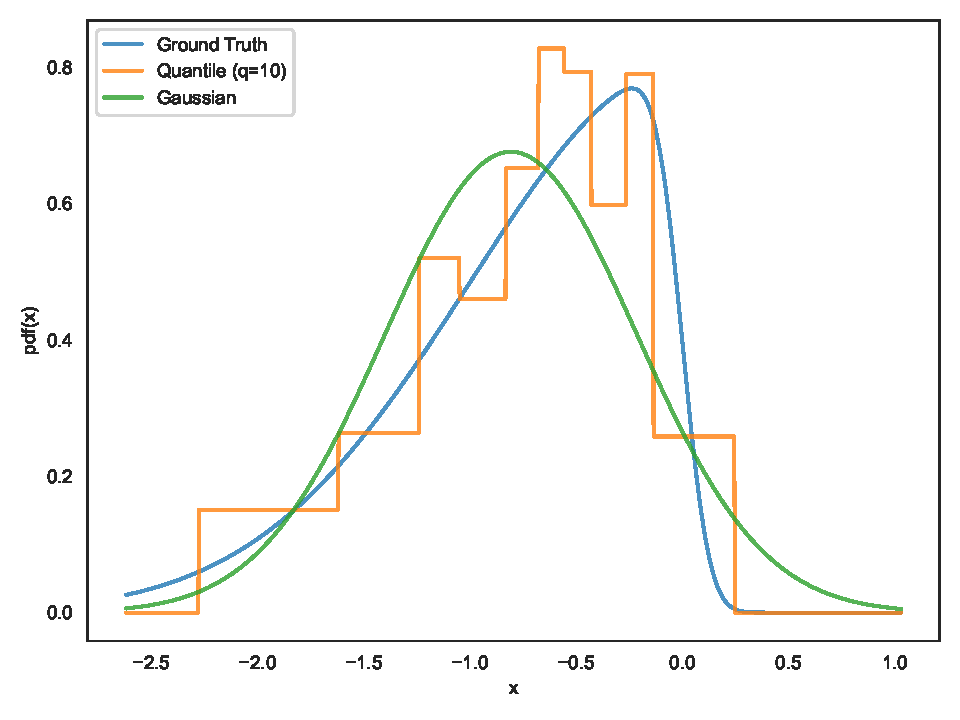
\includegraphics[width=\linewidth]{figs/10_pdf_plot.pdf}
    \\[0.5em]
    {\small (a)}
  \end{minipage}
  \hfill
  \begin{minipage}[b]{0.4\textwidth}
    \centering
    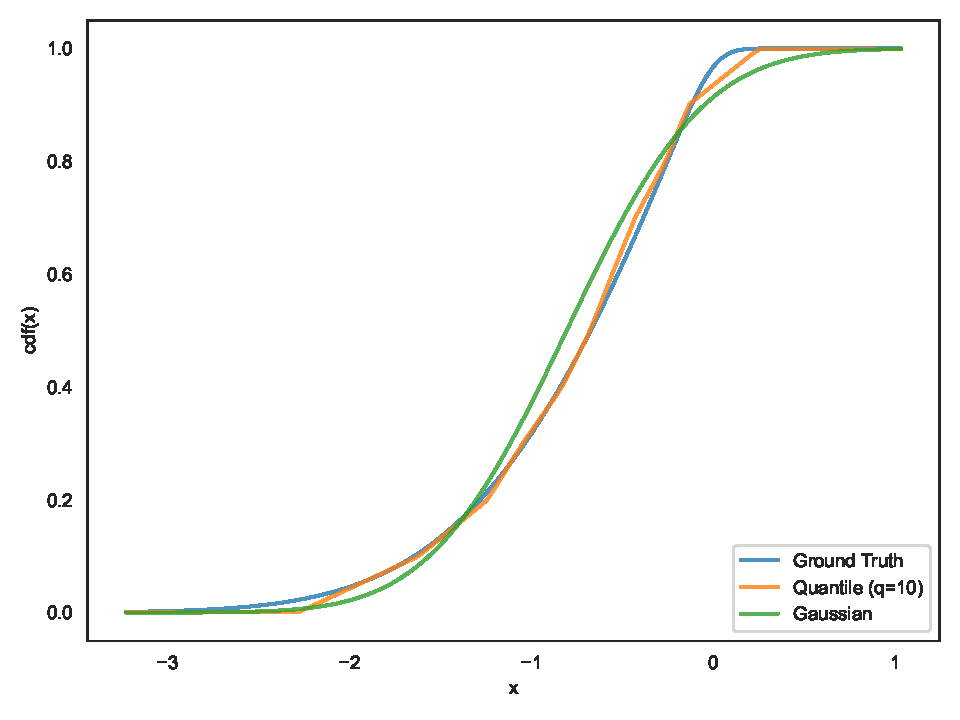
\includegraphics[width=\linewidth]{figs/10_cdf_plot.pdf}
    \\[0.5em]
    {\small (b)}
  \end{minipage}
  \hfill
   \begin{minipage}[b]{0.4\textwidth}
    \centering
    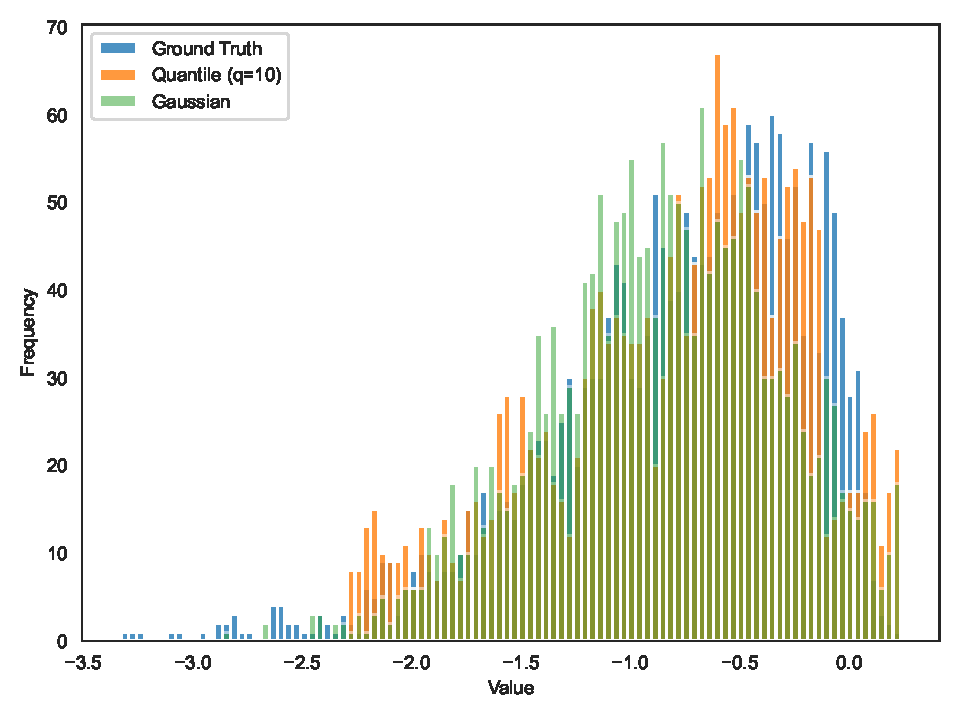
\includegraphics[width=\linewidth]{figs/10_rvs_plot.pdf}
    \\[0.5em]
    {\small (c)}
  \end{minipage}
 
 \vspace{1em}
 \parbox{\linewidth}{
 	 {\small \textit{Figure \ref{fig:distest10}:} Visualization of the distributions estimated from 10 quantile levels using a synthetic dataset with 150 samples. The figure includes the estimated \gls{pdf} (a), \gls{cdf} (b), and the histogram of 2000 samples drawn from the estimated distribution (c).}
 }
\end{figure}

% Second Row (20 Quantiles)
\begin{figure}[H]
  \refstepcounter{figure}
  \addcontentsline{lof}{figure}{Figure~\thefigure: Visualization of Estimated Distribution Based on 20 Quantiles.} 
  \label{fig:distest20}
  \centering
  \begin{minipage}[b]{0.4\textwidth}
    \centering
    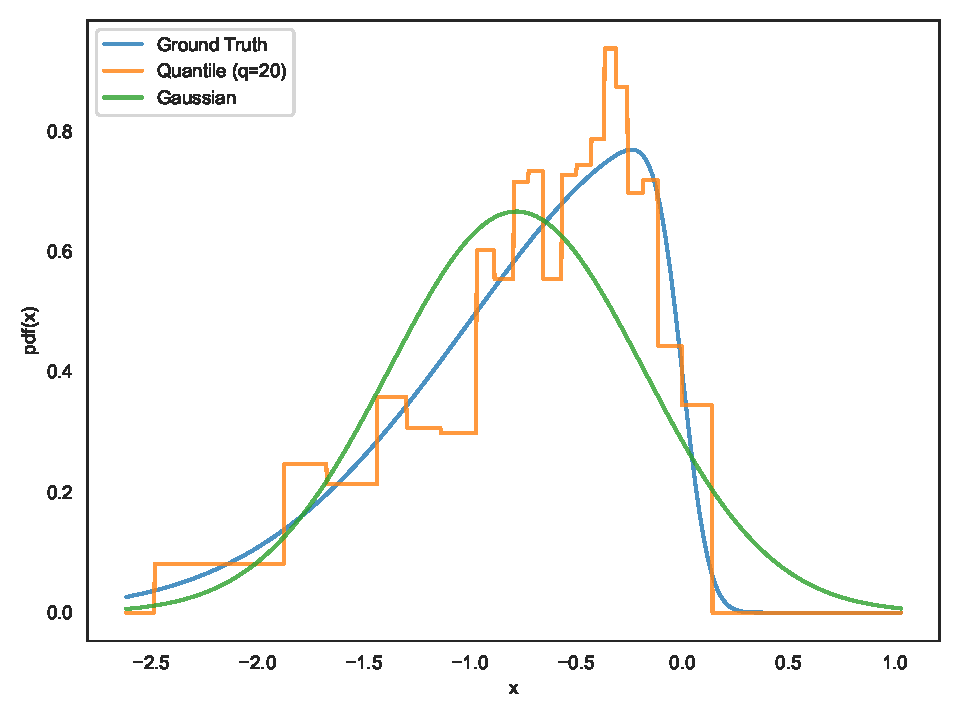
\includegraphics[width=\linewidth]{figs/20_pdf_plot.pdf}
    {\small (a)}
  \end{minipage}
  \hfill
  \begin{minipage}[b]{0.4\textwidth}
    \centering
    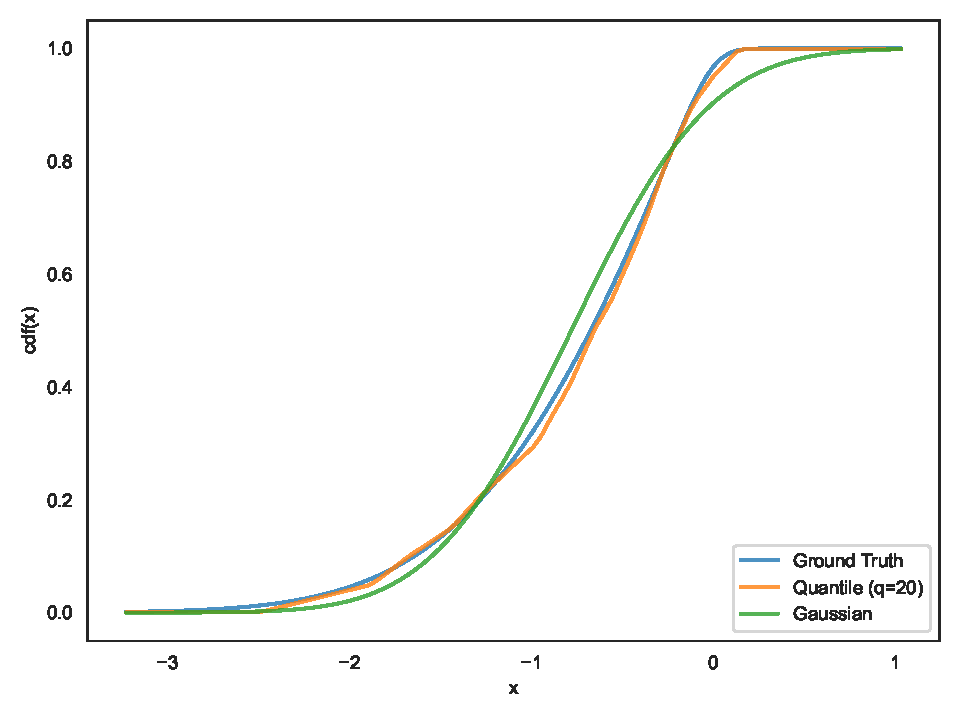
\includegraphics[width=\linewidth]{figs/20_cdf_plot.pdf}
    \\[0.5em]
    {\small (b)}
  \end{minipage}
  \hfill
   \begin{minipage}[b]{0.4\textwidth}
    \centering
    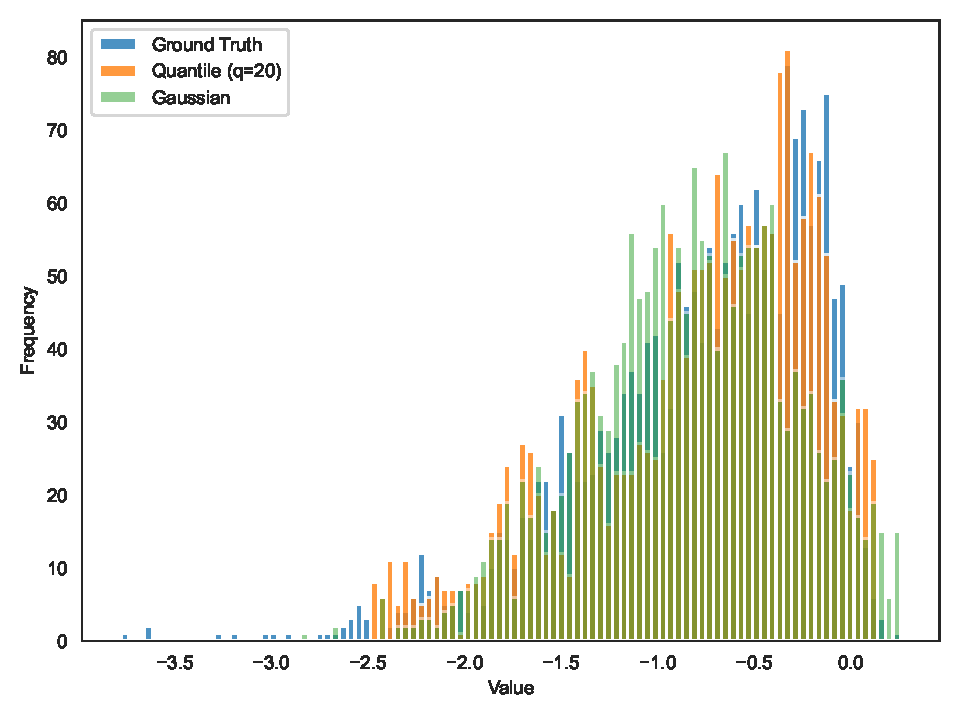
\includegraphics[width=\linewidth]{figs/20_rvs_plot.pdf}
    \\[0.5em]
    {\small (c)}
  \end{minipage}
  \vspace{1em}
  
 \parbox{\linewidth}{
 	 {\small \textit{Figure \ref{fig:distest20}:} Visualization of the distributions estimated from 20 quantile levels using a synthetic dataset with 150 samples. The figure includes the estimated \gls{pdf} (a), \gls{cdf} (b), and the histogram of 2000 samples drawn from the estimated distribution (c).}
 }
\end{figure}
\end{landscape}

\vspace{1em}
\section{Acquisition Function and Search Strategy}
\label{sec:acq}
Finally, we describe the acquisition functions and the aquisition optimization strategies used within the \gls{bananascp} framework.

\subsection{Acquisition Functions}
We consider four commonly used acquisition functions. Consistent with the notation in the previous sections, $\hat{f}(a)$ is the predicted performance of architecture $a$ and $\hat{F}_a$ represents the \gls{cdf} of the estimated distribution of $f(a)$. Then, depending on the acquisition function used, the specific acquisition score can be calculated by: 

\begin{description}[leftmargin=0cm, itemsep=1pt] 
\item[\gls{its}:] A sample is drawn from the distribution at random and its value is seen as the acquistion score for the candidate architecture $a$.
\item[\gls{ucb}:] The acquisition score is given by $\mu+\gamma \cdot \sigma$ for a Gaussian distribution, where $\gamma$ is the exploration factor. For non-Gaussian distributions, we follow \cite{deshpande2024online} and generalize the function to a quantile function, i.e., $\hat{F}^{-1}_a(\gamma)$.  As in the original formulation, higher values of $\gamma$ promotes exploration. In our experiments, we set $\gamma=0.75$ due to these concerns: a) the distribution of model performance is believed to be left-skewed; b) estimates of extreme quantiles are generally based on sparse observations and therefore might be less reliable. A value of 0.75 is likely to offer a reasonable trade-off between exploration and accurate estimation.
\item[\gls{pi}:] The probability of improvements corresponds to $1 - \hat{F}^{-1}_a(f_{max})$, with $f_{max}$ being the highest model performance ever observed.
\item[\gls{ei}:] The expected value of improvements can be written as $\mathbb{E}[\max(0,  f(a)- f_{max}})]$, with $f_{max}$ being the highest model performance ever observed. 
\end{description}

\vspace{0.3em}
\subsection{Acquisition Optimization Strategy}
In parallel to the settings in \cite{white2019bananas} (see Section \ref{sec:bananas}), we compare three different approaches for constructing a set with 100 \footnote{ We have conducted preliminary experiments using 1,000 candidate samples as well. The results indicate that increasing the sample size does not lead to significant improvements in performance. Considering the size of the search space (NAS-Bench-201), and the required computational time, the candidate set size is fixed at 100 for all subsequent primary experiments.} candidates in order to compute the acquisition scores. The motivations and the  specific approaches are described below:
 
\begin{description}[leftmargin=0cm, itemsep=1pt]
\item[Mutation] We investigate the mutation-based search strategy because this approach demonstrates the best performance in \cite{white2019bananas}. In line with their approach, the candidates are selected by randomly changing one operation or one edge of the $k$ best models that have been found so far, where $k$ is a search hyperparameter with the default value of 2. 
\item[Random Sampling] This approach is explored under the assumption that globally sampled architectures may improve the quality of the calibration process. As indicated by the name, the candidate set is created by randomly sampling architectures from the entire search space.
\item[Dynamic] This approach aims to resemble the "random + mutation" search strategy in \cite{white2019bananas}. The search process begins with random sampling until utilizing the first half of the search budget, then switches to a mutation-based strategy that progressively reduces the number of best ever-found models considered for mutation. To be precise, the number of models to be mutated decreases by 2 every 20 epoch. For instance, in a \gls{nas} task with 160 epochs, candidates are picked via random sampling for the first 80 epochs. Starting from epochs 80/100/120/140, the candidates are selected by mutating the best 8/6/4/2 models, respectively.
\end{description} 

